\subsection{Passarela de Sherbrooke, Canadá}
\label{chap:sher}

A passarela de Sherbrooke (\autoref{sherbrooke}), construída sobre o rio Magog, na cidade de Quebec, Canadá, foi a primeira estrutura construída inteiramente com concreto de pós reativos (CPR), uma variedade de concreto de ultra alto desempenho (CUAD), sem a utilização de barras de aço. Sua superestrutura consiste de treliças de CPR com com uma resistência característica de 200 MPa confinadas em tubos de aço inoxidável sobre um vão de 60 metros \cite[p.~140]{Aitcin_sher}.

\begin{figure}[htb]
	\caption{\label{sherbrooke}Passarela de Sherbrooke, Quebec, Canadá. Construída em CPR (concreto de pós reativos) sem o uso de barras de aço.}
	\begin{center}
	    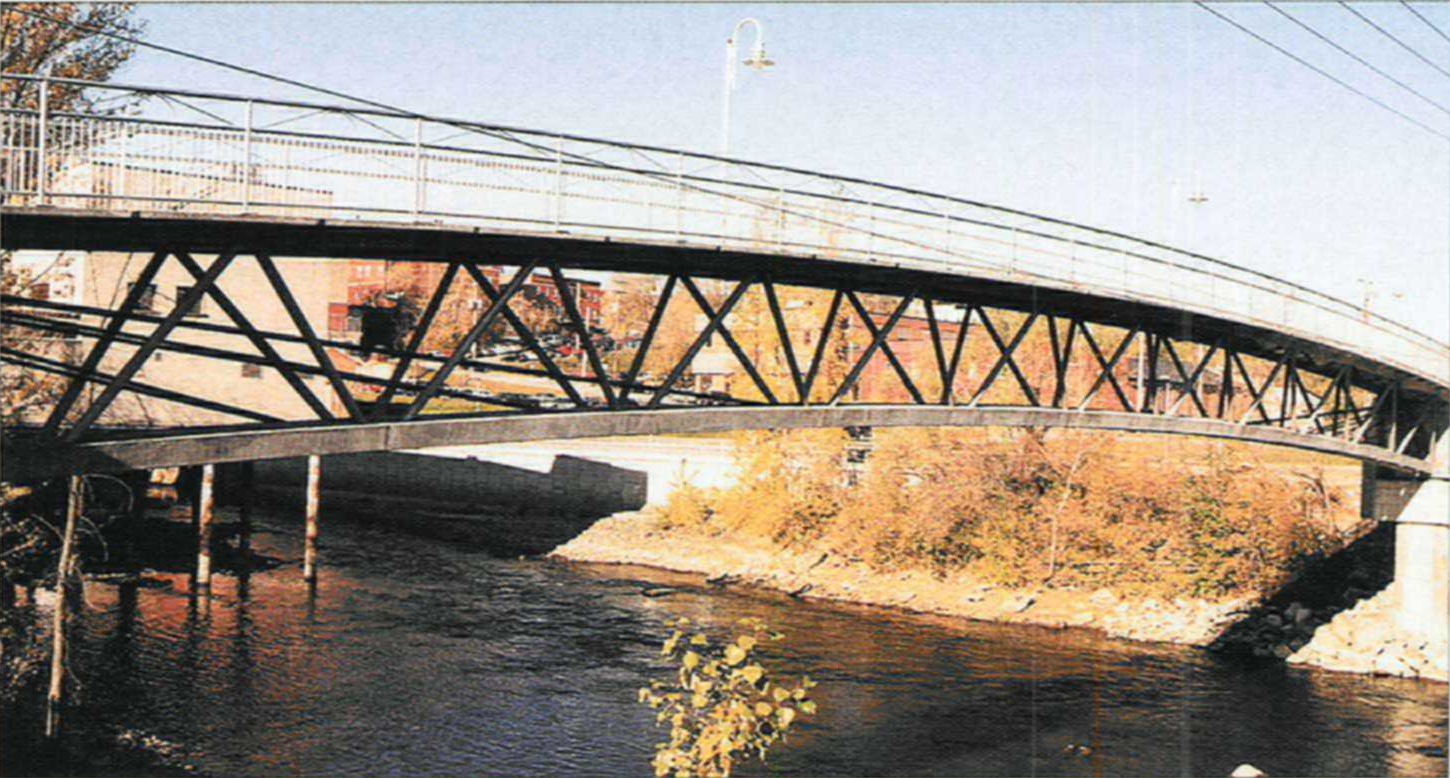
\includegraphics[max width=\textwidth]{sherbrooke.png}
	\end{center}
	\fonte{\citeonline[p.~140]{Aitcin_sher}.}
\end{figure}

As partículas utilizadas no CPR utilizado para construir a passarelas foram limitadas a 0,8 mm. Sua mistura consiste em cimento Portland, fumo de sílica, pó de quartzo, areia, superplastificante, água e fibras de aço com resistência de 2600 MPa, 0,2 mm de diâmetro e 13 mm de comprimento. A mistura foi confinada em tubos de aço inoxidável de 150 mm de diâmetro e espessura de 2 mm. Este confinamento serve para transformar a ruptura frágil apresentada pelo CUAD em uma ruptura pseudo-dúctil, além de melhorar ainda mais as suas propriedades mecânicas, incluindo a  capacidade de suportar uma solicitação de compressão de 350 MPa \citeonline[p.~141]{Aitcin_sher}. A \autoref{sherbrooke_traco} mostra o traço de CPR utilizado na passarela de Sherbrooke. Já a \autoref{sherbrooke_curva} mostra as curvas de tensão-deformação compressivas para diferentes tipos de concretos testados na época da construção da ponte. No gráfico, é possível observar um considerável aumento na resistência à compressão de um mesmo CPR em três condições distintas (livre, confinado e confinado e comprimido). A curva de tensão-deformação do CAD aparece apenas para se fazer um comparativo.

\begin{table}[htb]
\IBGEtab{%
  \caption{Dosagem do CPR usado na passarela de Sherbrooke.}
  \label{sherbrooke_traco}
}{%
  \begin{tabulary}{\linewidth}{CCC}
  \toprule
   Material                 & Quantidade    \\
  \midrule \midrule
   Cimento                  & 705 $\text{kg/m}^3$  \\ \midrule 
   Fumo de sílica           & 230 $\text{kg/m}^3$  \\ \midrule 
   Pó de quartzo            & 210 $\text{kg/m}^3$  \\ \midrule 
   Areia                    & 1010 $\text{kg/m}^3$ \\ \midrule 
   Superplastificante       & 37,5 $\text{l/m}^3$  \\ \midrule 
   Fibras de aço            & 190 $\text{kg/m}^3$  \\ \midrule 
   Água (a/c = 0,21)        & 195 $\text{l/m}^3$   \\
  \bottomrule
\end{tabulary}%
}{%
  \fonte{\citeonline[p.~141]{Aitcin_sher}.}%
  %\nota{Recomenda-se o uso de água de amassamento de baixa temperatura, pré cura térmica de 2 dias e cura térmica de 24 horas a uma temperatura de 80\textsuperscript{\degree} C.}
  %\nota[Anotações]{Uma anotação adicional, que pode ser seguida de várias outras.}
  }
\end{table}

\begin{figure}[htb]
	\caption{\label{sherbrooke_curva} Curvas de tensão-deformação compressivas para diferentes concretos.}
	\begin{center}
	    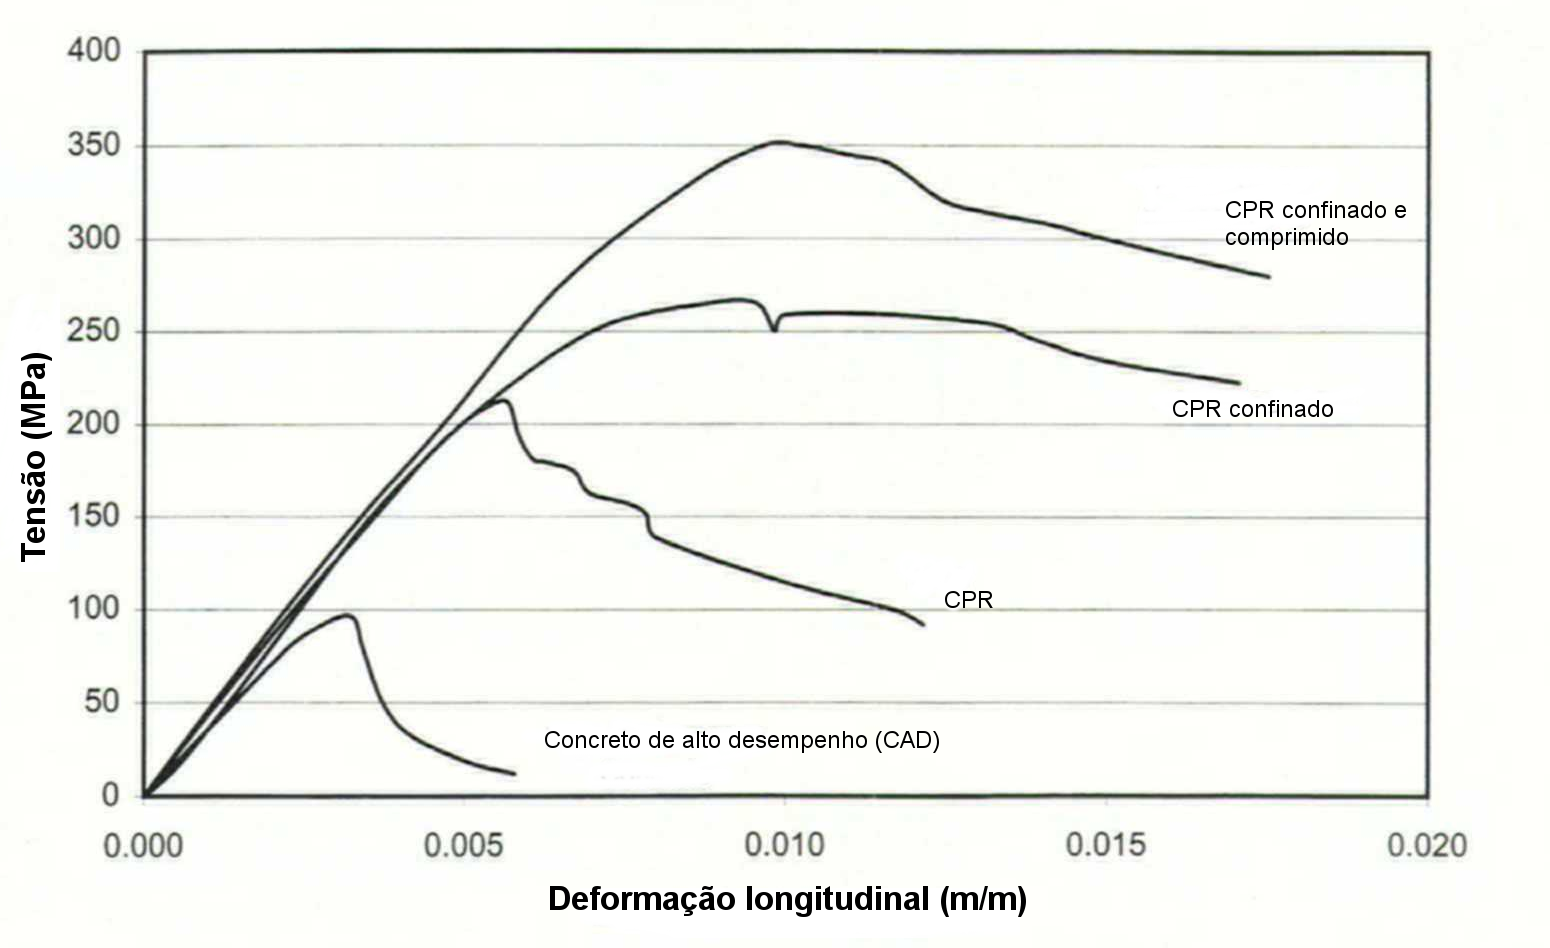
\includegraphics[max width=\textwidth]{sherbrooke-strain.png}
	\end{center}
	\fonte{\citeonline[p.~141]{Aitcin_sher}.}
\end{figure}

Para o projeto da passarela, foram feitas as seguintes considerações: resistência à compressão de 180 MPa, resistência à tração direta de 7 MPa, resistência à flexão de 40 MPa e módulo de elasticidade de 50 GPa. Através de um processo rigoroso de produção introduzido na fábrica de pré-moldados onde a passarela foi moldada, compressão do CPR ainda fresco e cura térmica a vapor, a uma temperatura de 90\textsuperscript{\degree} C, o material foi capaz de atingir uma resistência média de 200 MPa, aferida em corpos de prova recolhidos em diferentes lotes de produção de CPR \cite[p.~141]{Aitcin_sher}.

A passarela possui um tabuleiro de 30 mm de espessura, protendido transversalmente e longitudinalmente e não possui reforço passivo de aço. Por motivos de segurança, o potencial do material não foi explorado completamente, já que esta foi a primeira experiência de uso do material em uma obra aberta ao público \cite[p.~141]{Aitcin_sher}. A seção transversal e longitudinal pode ser vista na \autoref{cross-section} e na \autoref{longitudinal}, respectivamente. A \autoref{precast} mostra um segmento pré-moldado finalizado da ponte, ainda na fábrica.

\begin{figure}[htb]
	\caption{\label{cross-section} Corte transversal da passarela de Sherbrooke.}
	\begin{center}
	    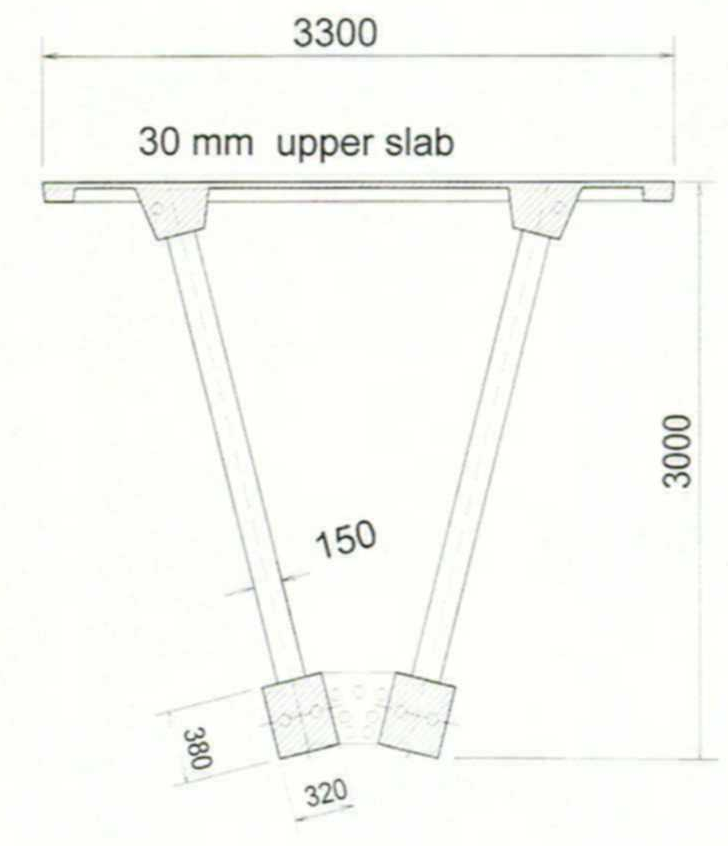
\includegraphics[max width=4cm]{cross-section.png}
	\end{center}
	\fonte{\citeonline[p.~141]{Aitcin_sher}.}
\end{figure}

\begin{figure}[htb]
	\caption{\label{longitudinal}Elevação da passarela de Sherbrooke mostrando a protensão longitudinal.}
	\begin{center}
	    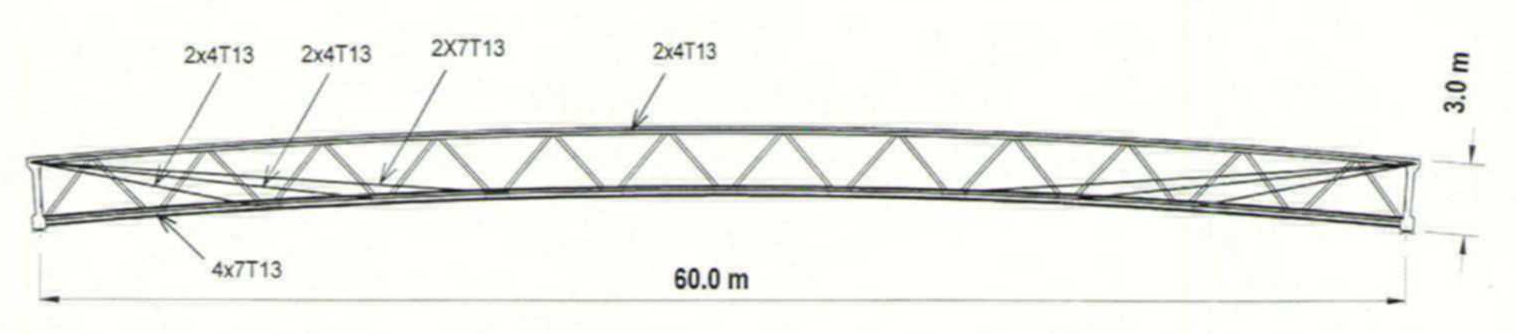
\includegraphics[max width=\textwidth]{longitudinal-prestressing.png}
	\end{center}
	\fonte{\citeonline[p.~142]{Aitcin_sher}.}
\end{figure}

\begin{figure}[htb]
	\caption{\label{precast}Segmento pré-moldado finalizado da passarela.}
	\begin{center}
	    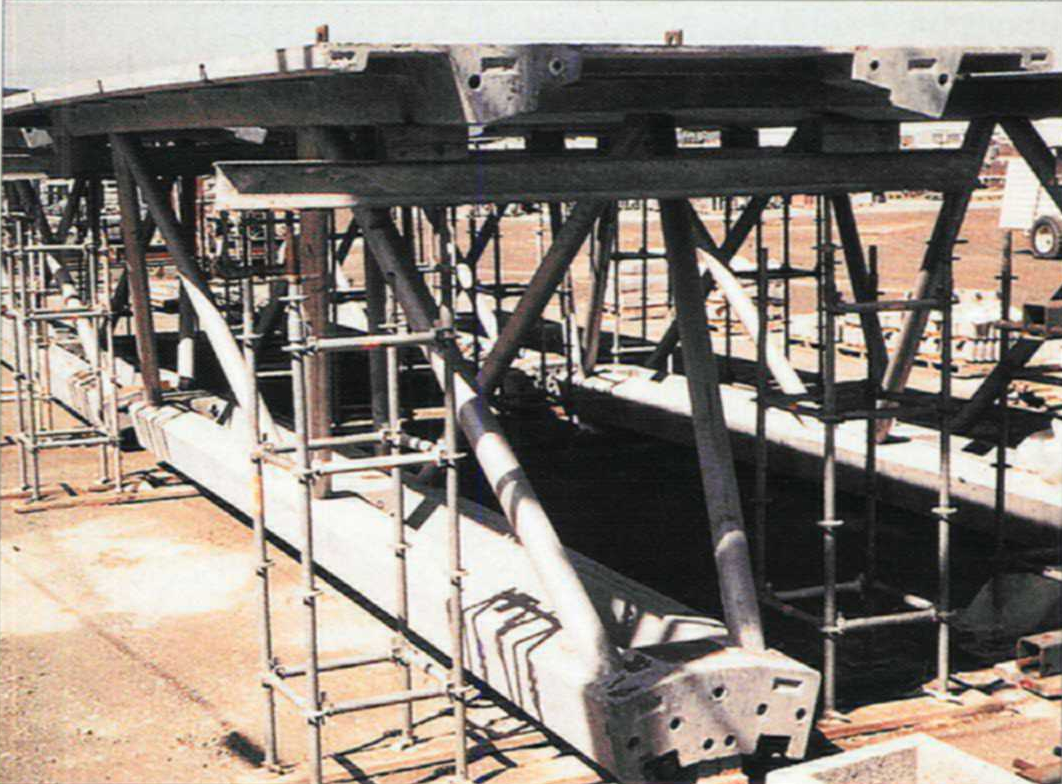
\includegraphics[max width=\textwidth]{precast.png}
	\end{center}
	\fonte{\citeonline[p.~142]{Aitcin_sher}.}
\end{figure}